\documentclass[border=10pt]{standalone}
\usepackage{tikz}\usepackage{amsmath}
\usetikzlibrary{calc,arrows.meta}
\begin{document}
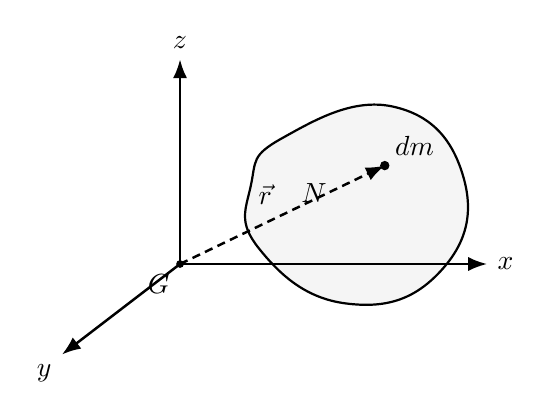
\begin{tikzpicture}[line width=0.9pt,>={Latex[length=2.4mm]}]
  % cuerpo (blob)
  \draw[thick,fill=black!4] plot[smooth cycle,tension=0.8] coordinates
    {(1.3,1.6)(2.7,2.0)(3.6,1.1)(3.3,-0.1)(2.1,-0.5)(1.0,0.2)(0.9,1.0)};
  \node at (1.7,0.9){$N$};
  % ejes desde G
  \coordinate (G) at (0,0);
  \draw[->] (G) -- (3.9,0) node[right]{$x$};
  \draw[->] (G) -- (0,2.6) node[above]{$z$};
  \draw[->] (G) -- (-1.5,-1.15) node[below left]{$y$};
  \fill (G) circle(1.4pt) node[below left]{$G$};
  % elemento de masa dm
  \coordinate (P) at (2.6,1.25);
  \fill (P) circle(1.7pt) node[above right]{$dm$};
  \draw[->,densely dashed] (G) -- (P) node[midway,above left]{$\vec r$};
\end{tikzpicture}
\end{document}
